\subsection{UX diagrams}

To provide a complete understanding of how the user interfaces are designed, both for the web application, the mobile application and the on-board software, user experience diagrams are provided in the following.

The user interface for the customers [figure \ref{fig:device-ux}] and the system's administrators [figure \ref{fig:admin-ux}] are different since the functionalities provided them are design according to their relation with the system. This difference is here shown by the corresponding UX diagrams.

It's worth noting that the user interface for the web application and the mobile application share the same design, since the mobile application is only a mobile optimization of the former.

In order to keep the diagrams as clean and simple as possible, the Logout and Homepage navigation links are not displayed. It's assumed that every screen containing the logout() and homepage() functionalities refers, respectively, to the Logout screen and Logged Homepage screen.

\begin{figure}[H]
	\centerline{
		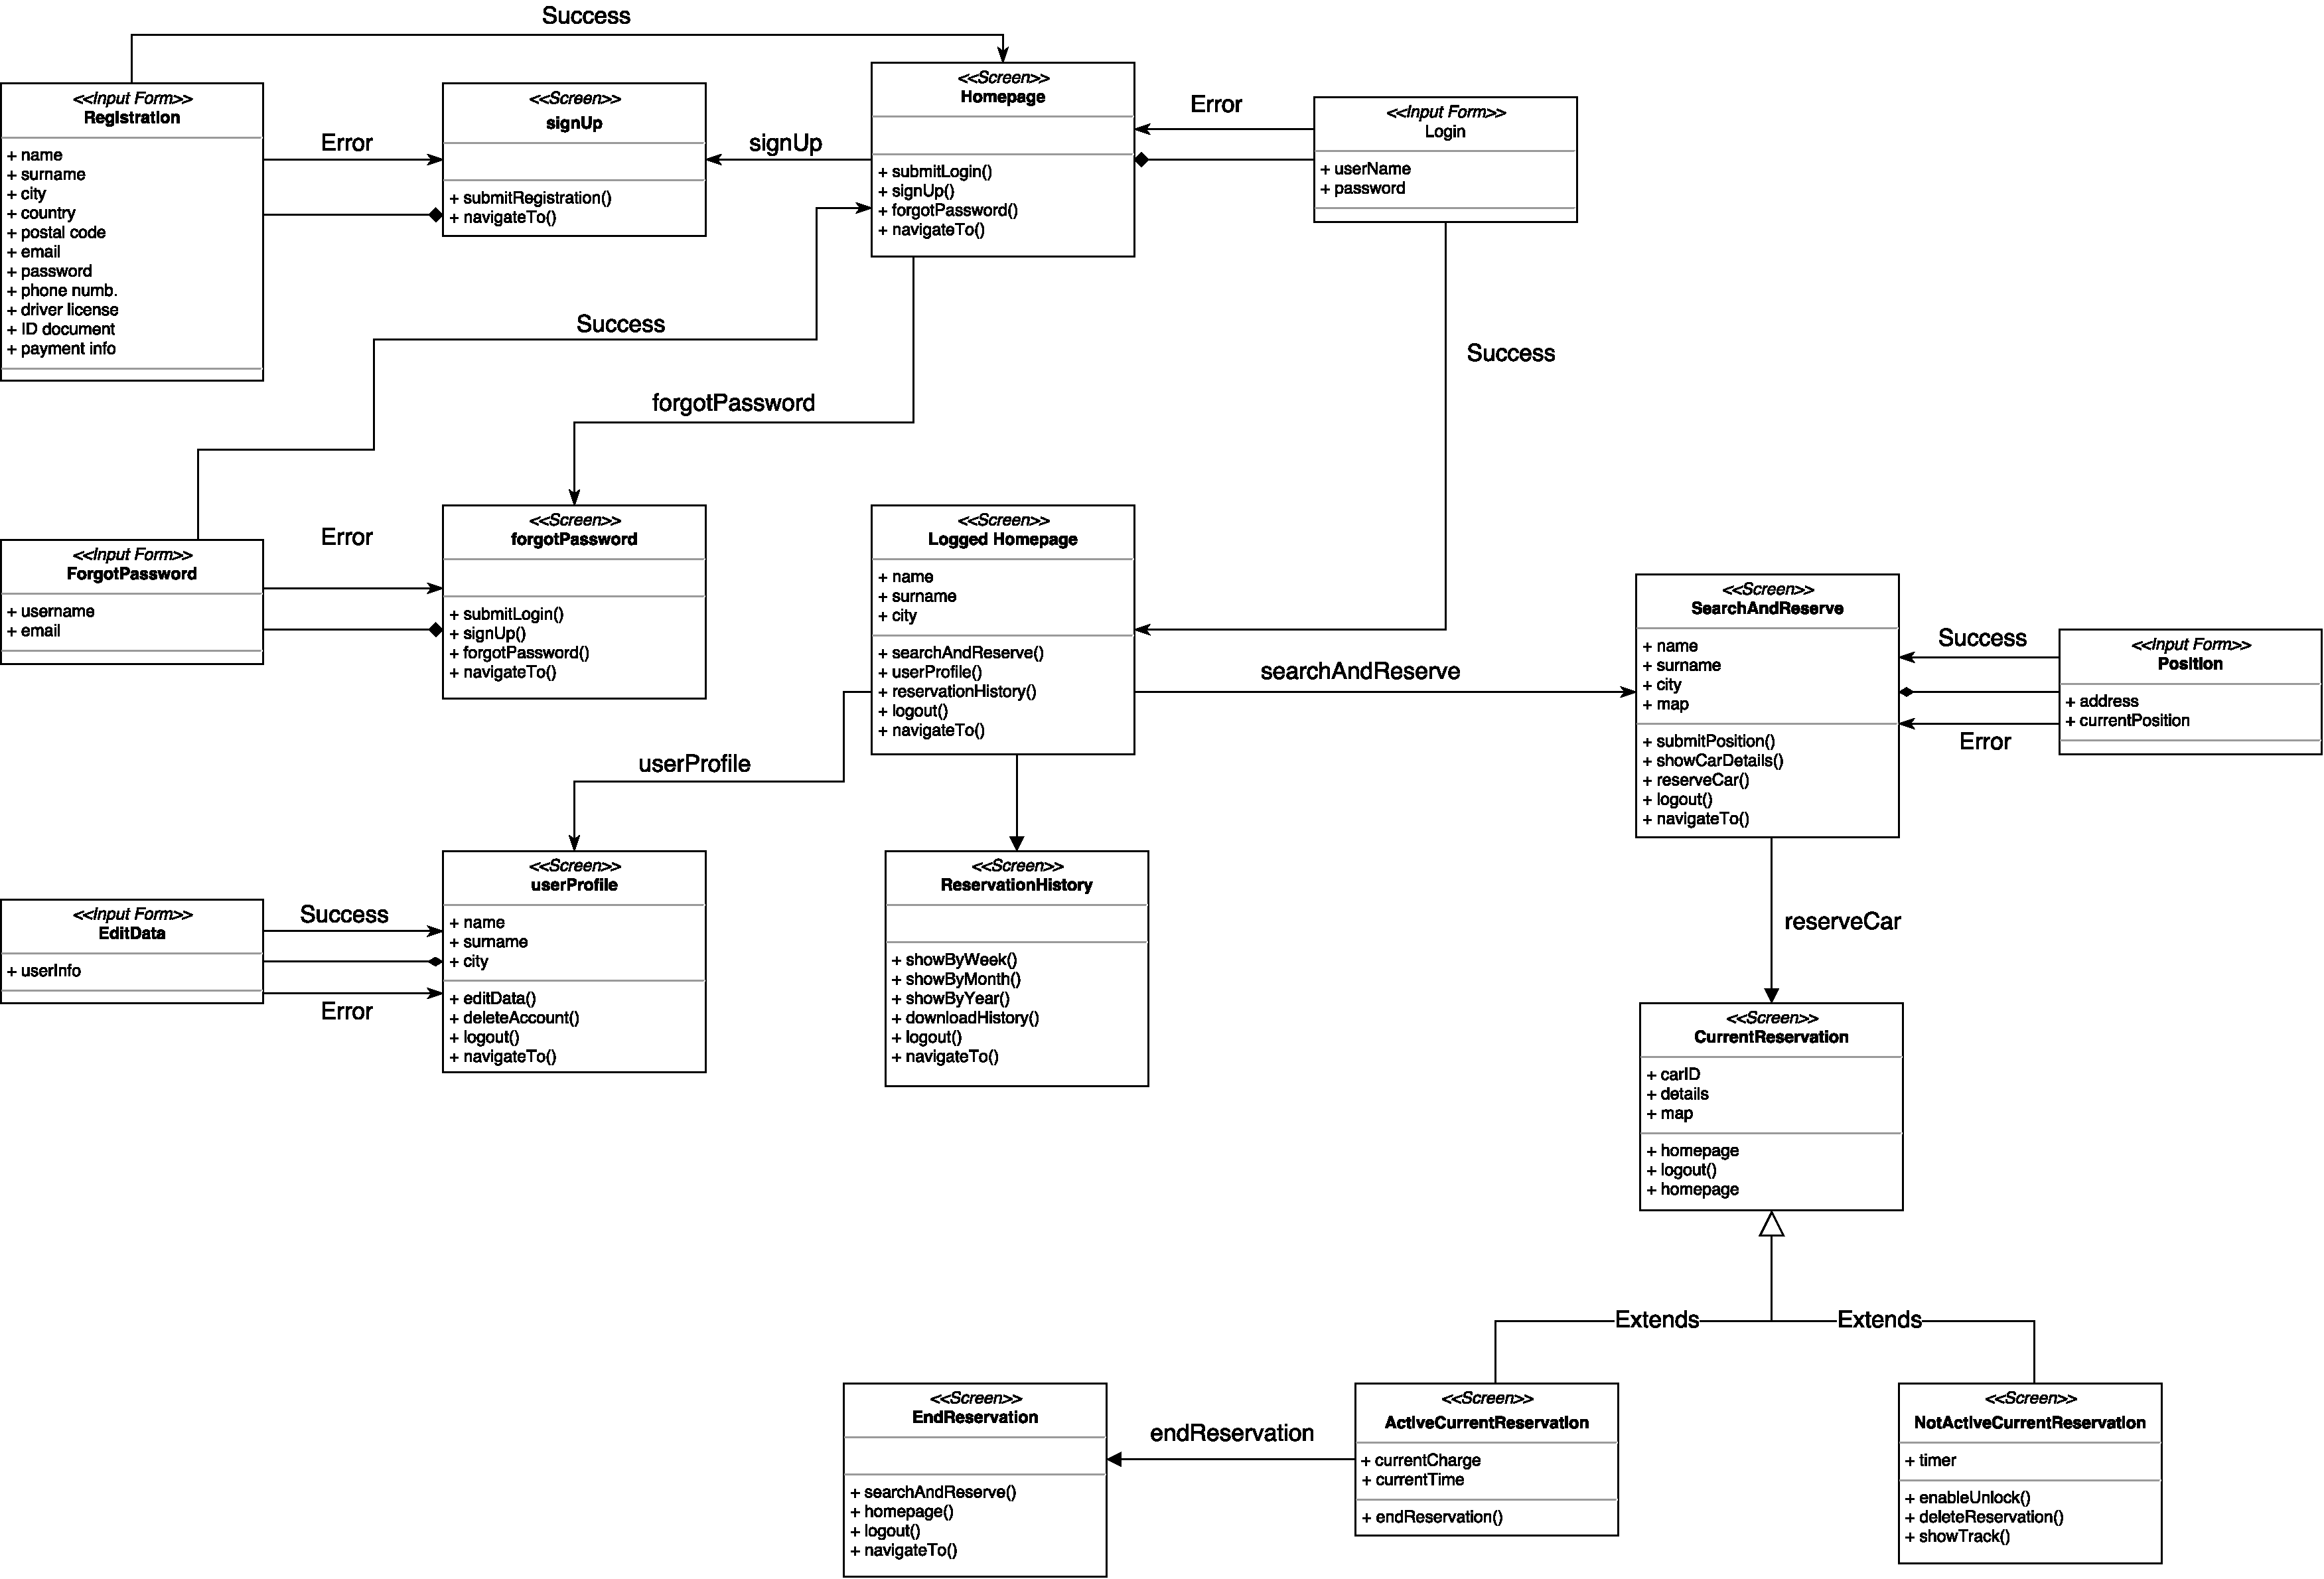
\includegraphics[width=400px]{../Datas/images/deviceUX.pdf}
	}
	\caption{Web application \& Mobile application UX}
	\label{fig:device-ux}
\end{figure}

\begin{figure}[H]
	\centerline{
		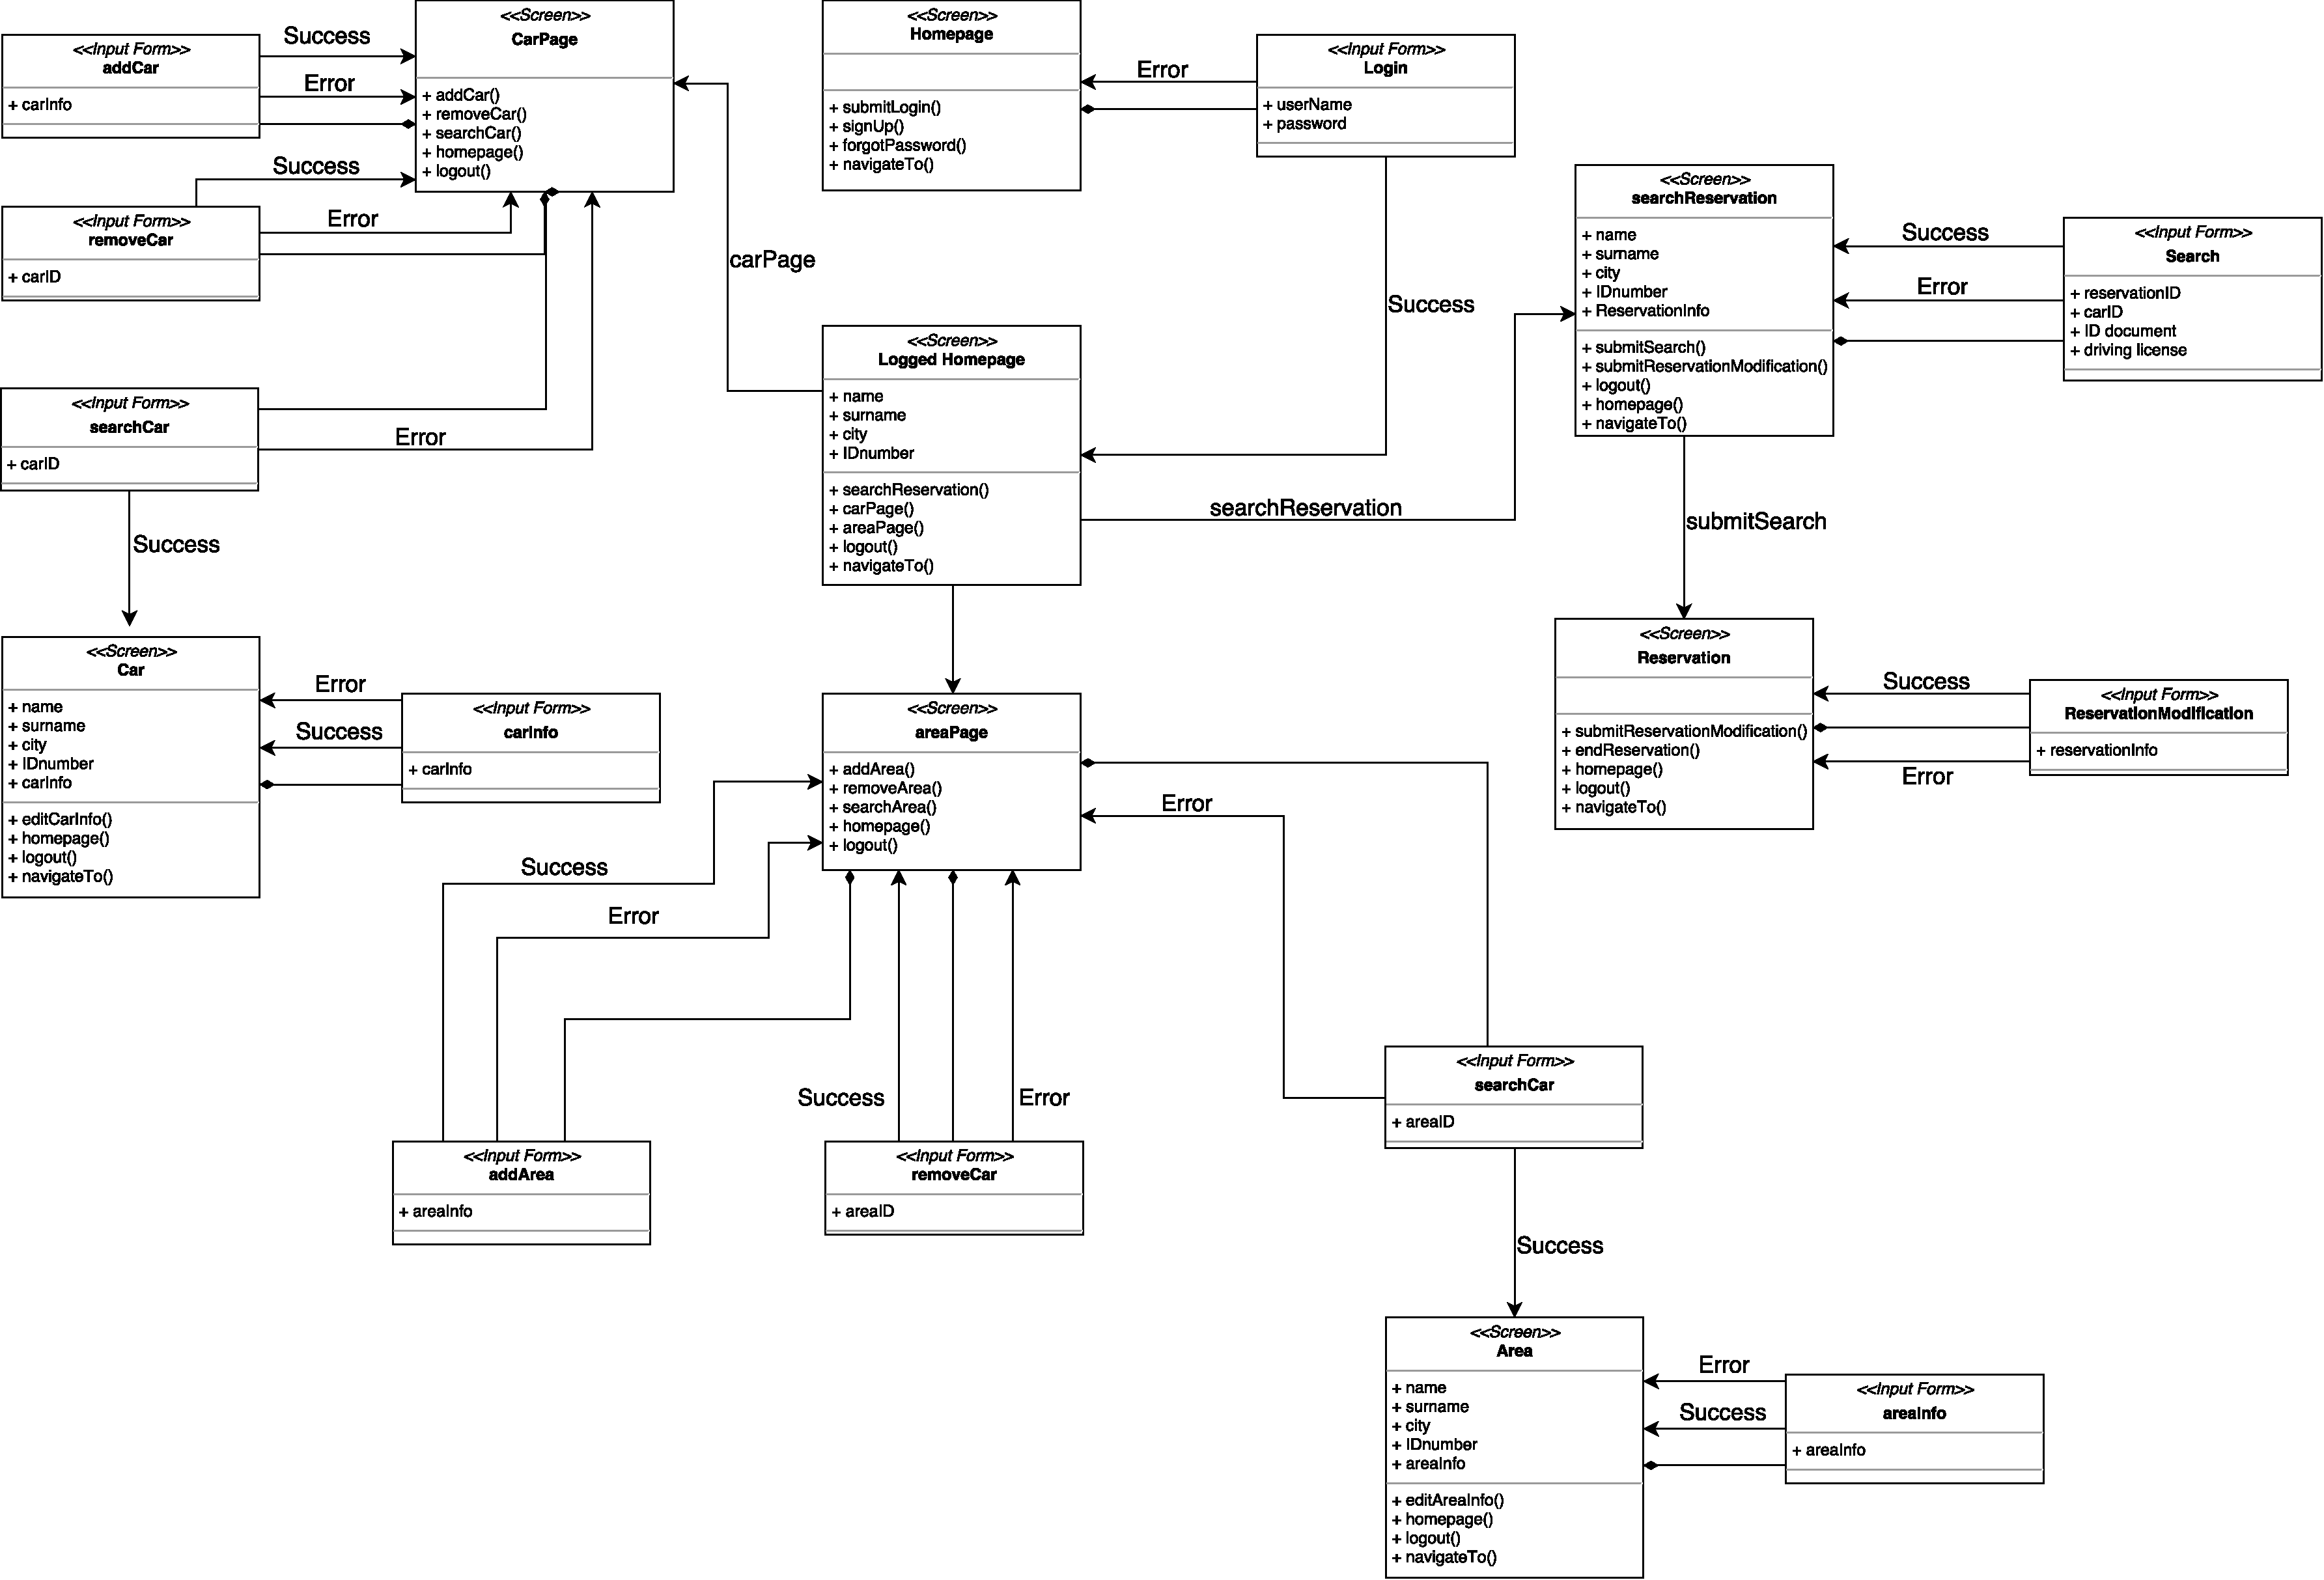
\includegraphics[width=400px]{../Datas/images/UXoperator.pdf}
	}
	\caption{Administrator UX}
	\label{fig:admin-ux}
\end{figure}

\begin{figure}[H]
	\centerline{
		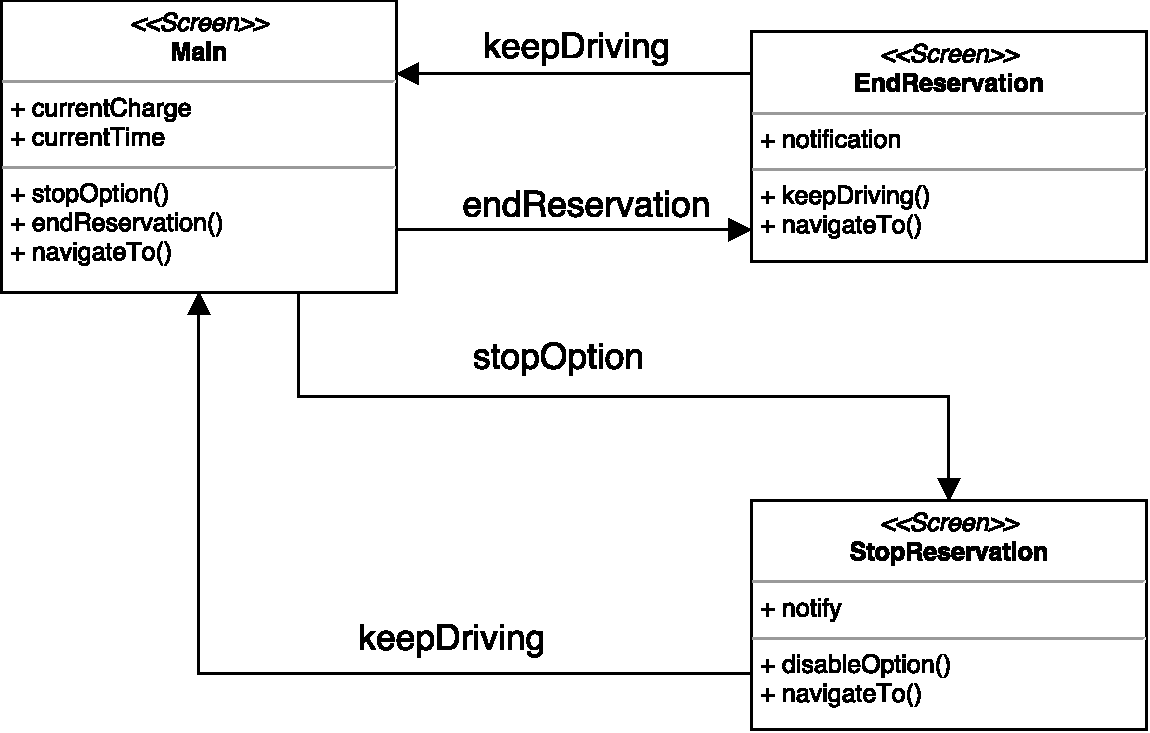
\includegraphics[width=250px]{../Datas/images/carDisplayUX.pdf}
	}
	\caption{On-board software UX}
	\label{fig:car-ux}
\end{figure}
